%% Copernicus Publications Manuscript Preparation Template for LaTeX Submissions
%% ---------------------------------
%% This template should be used for copernicus.cls
%% The class file and some style files are bundled in the Copernicus Latex Package, which can be downloaded from the different journal webpages.
%% For further assistance please contact Copernicus Publications at: production@copernicus.org
%% https://publications.copernicus.org/for_authors/manuscript_preparation.html


%% Please use the following documentclass and journal abbreviations for preprints and final revised papers.

%% 2-column papers and preprints
\documentclass[gmd, manuscript]{copernicus}



%% Journal abbreviations (please use the same for preprints and final revised papers)


% Advances in Geosciences (adgeo)
% Advances in Radio Science (ars)
% Advances in Science and Research (asr)
% Advances in Statistical Climatology, Meteorology and Oceanography (ascmo)
% Aerosol Research (ar)
% Annales Geophysicae (angeo)
% Archives Animal Breeding (aab)
% Atmospheric Chemistry and Physics (acp)
% Atmospheric Measurement Techniques (amt)
% Biogeosciences (bg)
% Climate of the Past (cp)
% DEUQUA Special Publications (deuquasp)
% Earth Surface Dynamics (esurf)
% Earth System Dynamics (esd)
% Earth System Science Data (essd)
% E&G Quaternary Science Journal (egqsj)
% EGUsphere (egusphere) | This is only for EGUsphere preprints submitted without relation to an EGU journal.
% Earth Observation (eo)
% European Journal of Mineralogy (ejm)
% Geochronology (gchron)
% Geographica Helvetica (gh)
% Geoscience Communication (gc)
% Geoscientific Instrumentation, Methods and Data Systems (gi)
% Geoscientific Model Development (gmd)
% History of Geo- and Space Sciences (hgss)
% Hydrology and Earth System Sciences (hess)
% Journal of Bone and Joint Infection (jbji)
% Journal of Environmentally Compatible Air Transport System (jecats)
% Journal of Micropalaeontology (jm)
% Journal of Sensors and Sensor Systems (jsss)
% Magnetic Resonance (mr)
% Mechanical Sciences (ms)
% Natural Hazards and Earth System Sciences (nhess)
% Nonlinear Processes in Geophysics (npg)
% Ocean Science (os)
% Polarforschung - Journal of the German Society for Polar Research (polf)
% Proceedings of the International Association of Hydrological Sciences (piahs)
% Proceedings of the International Ocean Drilling Programme (piodp)
% Safety of Nuclear Waste Disposal (sand)
% Scientific Drilling (sd)
% SOIL (soil)
% Solid Earth (se)
% State of the Planet (sp)
% The Cryosphere (tc)
% Weather and Climate Dynamics (wcd)
% Web Ecology (we)
% Wind Energy Science (wes)


%% \usepackage commands included in the copernicus.cls:
%\usepackage[german, english]{babel}
%\usepackage{tabularx}
%\usepackage{cancel}
%\usepackage{multirow}
%\usepackage{supertabular}
%\usepackage{algorithmic}
%\usepackage{algorithm}
%\usepackage{amsthm}
%\usepackage{float}
%\usepackage{subfig}
%\usepackage{rotating}


\begin{document}

\title{Diagnostic Specific Language for the Energy Exascale Earth System Model}


% \Author[affil]{given_name}{surname}

\Author[1][naser.mahfouz@pnnl.gov]{Naser}{Mahfouz} %% correspondence author
\Author[2]{Luca}{Bertagna}
\Author[3]{Aaron}{Donahue}
\Author[4]{Peter}{Schwartz}
\Author[5]{Jeffrey}{Johnson}
\Author[6]{Noel}{Keen}
\Author[3]{Hassan}{Beydoun}
\Author[2]{Benjamin}{Hillman}
\Author[3]{Walter}{Hannah}
\Author[3]{Peter}{Bogenschutz}
\Author[1]{Johannes}{M\"ulmentst\"adt}
\Author[7]{More}{Friends}

\affil[1]{Pacific Northwest National Laboratory, Richland, WA, USA}
\affil[2]{Sandia National laboratories, Albuquerque, NM, USA}
\affil[3]{Lawrence Livermore National Laboratory, Livermore, CA, USA}
\affil[4]{Oak Ridge National Laboratory, Oak Ridge, TN, USA}
\affil[5]{Cohere Consulting LLC, Seattle, WA, USA}
\affil[6]{Lawrence Berkeley National Laboratory, Berkeley, CA, USA}
\affil[7]{Somewhere on This Bitter Earth, Anywhere, SW, TBE}

%% The [] brackets identify the author with the corresponding affiliation. 1, 2, 3, etc. should be inserted.

%% If an author is deceased, please add \deceased[$Deceased date if applicable$]{$Author number$} (e.g. \deceased[13 November 2015]{2}) at the end of the affiliations. The author number depends on the placement of the author in the author list, e.g. the third author has number 3.


%% If authors contributed equally, please add \equalcontrib{$Author numbers$} (e.g. \equalcontrib{1,3}) at the end of the affiliations. The author number depends on the placement of the author in the author list, e.g. the third author has number 3.




\runningtitle{Diagnostic Specific Language for E3SM}

\runningauthor{Mahfouz et al.}





\received{}
\pubdiscuss{} %% only important for two-stage journals
\revised{}
\accepted{}
\published{}

%% These dates will be inserted by Copernicus Publications during the typesetting process.


\firstpage{1}

\maketitle



\begin{abstract}
Our thesis: We argue diagnostics are mathematical expressions represented by flexible
compositions of a small set of operators and an algebra over them
and that they should be evaluated by the model at runtime.
The result: A scientist can imagine a variable or product and \emph{project} it out
in a variety of productive ways --- instantaneous or averaged, over an arbitrary time period,
mapped, masked, or redefined --- without touching the source code.
\end{abstract}

\introduction  %% \introduction[modified heading if necessary]

\subsection{Diagnostics in ESMs}
Legacy paradigm: developer-scientists hard-code a fixed menu of diagnostics; everything else is done offline from raw output/archive.
Adequate for coarse-resolution and/or monthly climatologies. Not scalable/responsive to high-res and high-freq.

\subsection{Why higher-res/higher-freq breaks it}
The cost of writing raw state at the frequency the science needs grows exponentially. Post-processing stops being cheap and starts being the bottleneck.
Some diagnostics (e.g., conditional moments) are simply intractable offline at high resolution.

\subsection{Two responses/options}
\begin{enumerate}
  \item Incremental/streaming: keep the legacy outputs and get cleverer about moving and compressing them.
  \item Fundamental: push the diagnostic computation into the runtime, minimize I/O, and expose a composable vocabulary.
\end{enumerate}

Broadly, option 1 is the direction of everyone (including the European centers).
E3SM's C++ atmosphere has been taking option 2 incrementally for two years without naming it.
This manuscript names it, and we propose to formalize it.

\subsection{Scope of this paper}
We describe what the E3SM atmosphere does today, argue that it already constitutes a
diagnostics-specific language, show a gallery of science it enables.
We close by arguing for generalizing it across the model.


\section{Diagnostics in EAMxx today}
History and orientation: new model, new language, new runtime, etc. inspired a new way of doing stuff.
Explain the software philosophy at the outset.

\subsection{The diagnostic abstraction}
A diagnostic declares its input fields as data, is handed them by the orchestrator, and
produces one or more output fields.
Lazily evaluated and timestamp-cached, so shared subexpressions
compute once.
Registration through a factory.

\subsection{The operator algebra}
List/table what we have:
vertical extraction (levels, pressure, height);
horizontal reduction (global, zonal bins);
vertical reduction (sum/avg, mass- and thickness-weighted);
vertical derivatives;
time operators/management (instantaneous, average, accumulate, reset, etc.);
binary/unary arithmetics;
conditional sampling;
histograms;
simulators;
named physical diagnostics.
The algebra is closed: operators consume fields and produce fields, so they chain/compose (if they respect the expected input/output conventions).

\subsection{Surface syntax and the parser}
Tell story of slow beginnings, then formalization through a proper grammar, opting for xarray-inspired syntax.
\begin{verbatim}
((omega*qv).derivative(dx=dz,dims=['col'])).where(omega <= -10)
\end{verbatim}

\subsection{Multi-output diagnostics, caching, and (instrument) simulators}

\subsection{Evaluation: from yaml entry to variable on disk}


\subsection{Caveats and rough edges}
We force users to know grids, layouts, and (si) units for now.

\section{Gallery: science we did not plan for}
{The central evidence for the thesis. Each subsection: the scientific question, the expression
the user wrote, what it would have cost under the legacy paradigm, and --- critically --- the fact
that it was a byproduct of the software philosophy rather than a designed feature.}

\subsection{Horizontal and vertical reductions; e.g., RCE sims}

\subsection{Arbitrary slice reductions; e.g., cloud-top quantities}

\subsection{Conditional moments and correlations: e.g., Cess2}
{Capturing $\overline{uv}$ instead of $\overline{u}\,\overline{v}$ without storing the full high-frequency state.}

\subsection{Instability and oscillatory surface analyses; e.g., surface coupling}

\section{Costs and benefits}

\subsection{Runtime cost versus I/O cost}
A few benchmarks

\subsection{Minimizing regrets: the fear of missing/forgetting data}
The rational objection is ``what if I did not ask for the right thing because I couldn't have possibly anticipated wanting to analyze xyz phenomena?''
Responses: raw output is still available to anyone who wants it; saving well-chosen \emph{intermediates} can also help; and the regret space will shrink as the algebra space expands.

\subsection{Relationship to streaming and compression}
All these are complementary, not competitive.


\section{Toward a general and unified diagnostics language}


\begin{figure}
    \centering
    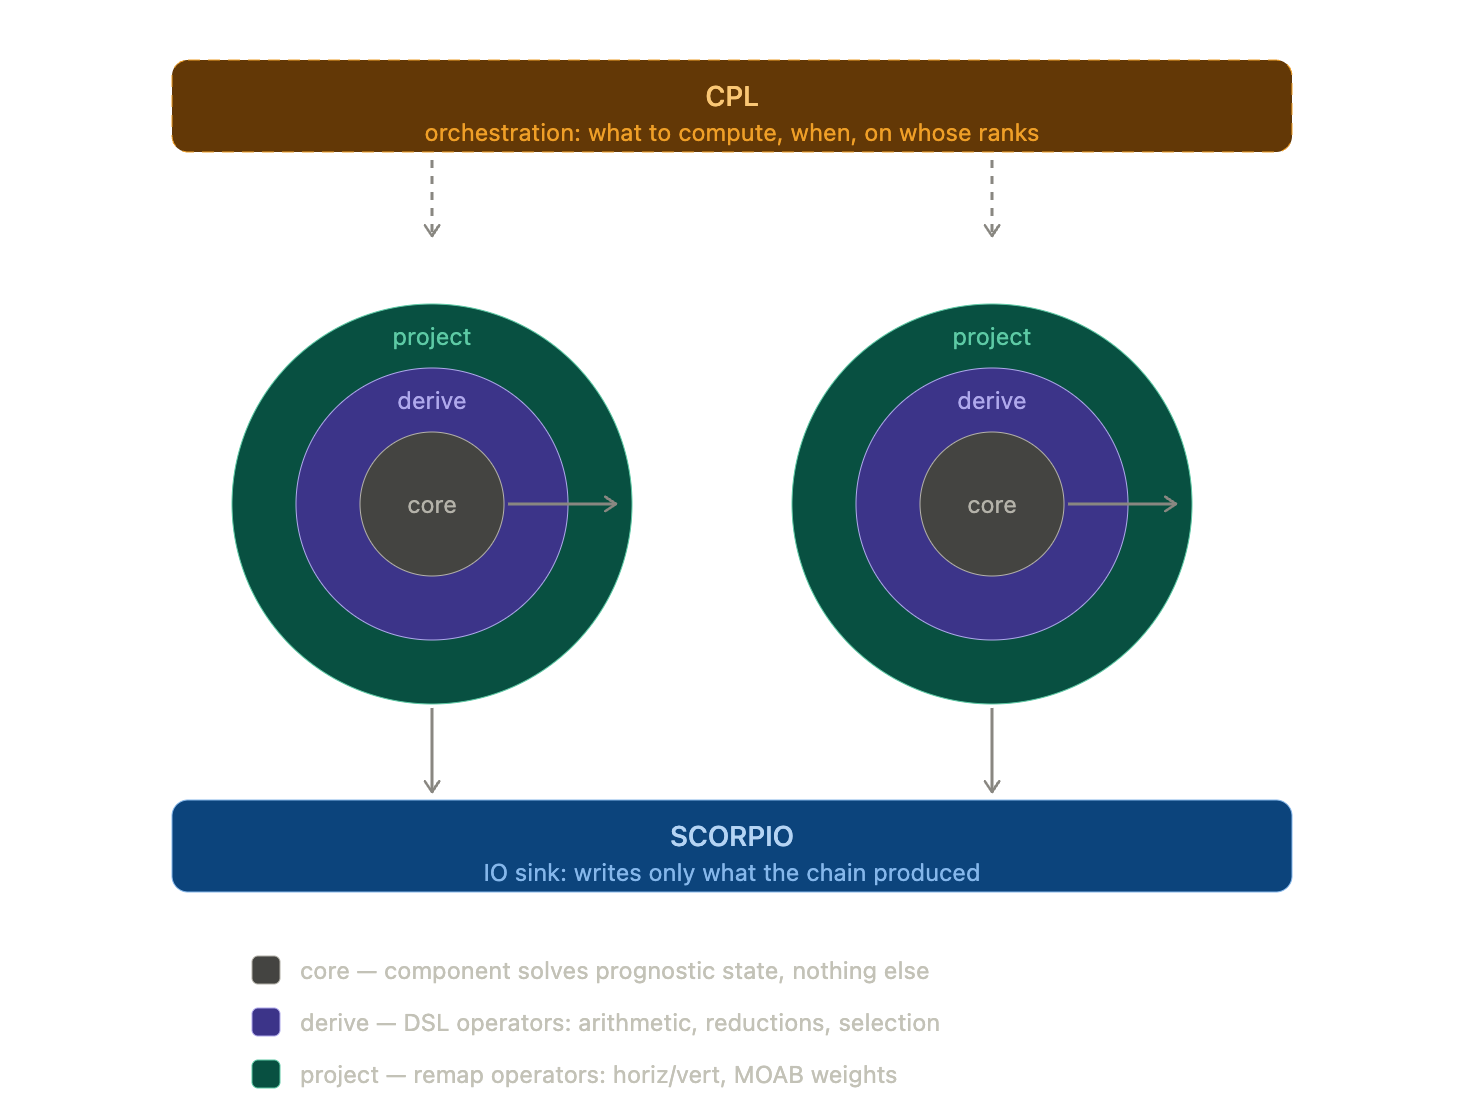
\includegraphics[width=.75\linewidth]{../fig/concentric-shells.png}
    \caption{A vision for a future E3SM of lots of shared cores, but thin interfaces in each component ...}
    \label{fig:placeholder}
\end{figure}

\subsection{The principles, stated plainly}

\begin{enumerate}
  \item Diagnostics should not be hard-coded.
  \item They should be parsed at runtime, and evaluated where the data already lives (on the GPU).
  \item They should be flexible and composable --- small operators, closed algebra.
  \item They should be arbitrarily projectable.
  \item They should be useful for science and hypothesis testing.
  \item They should be useful for logistics, e.g.\ saving disk space.
  \item They should be useful for extensions, e.g.\ AI/hybrid modeling.
\end{enumerate}

\subsection{Generalization: what is atmosphere-specific and what is not}
How to deal with component-specific conventions and extrapolate.

\subsection{Unification vision: a shared core with component-specific shells}
The concentric-shell picture: a shared parser, a kernelizer and kernel library, and a base driver, with component drivers building on top for their own needs.
Components adopt rather than reinvent.

\subsection{Implications for the AI era}
Emulator-ready outputs by construction; hybrid and online-learning workflows; the longer-term
``kernelizer'' idea of generating kernels on the fly from human-readable expressions.

\subsection{A counterpoint to the prevailing winds}


\conclusions  %% \conclusions[modified heading if necessary]
Philosophy of software innovation enables more science than it was designed to do, and a productive cycle of science/software co-evolution...

%% The following commands are for the statements about the availability of data sets and/or software code corresponding to the manuscript.
%% It is strongly recommended to make use of these sections in case data sets and/or software code have been part of your research the article is based on.


\codedataavailability{TEXT} %% use this section when having data sets and software code available




\appendix
\section{}    %% Appendix A

\subsection{}     %% Appendix A1, A2, etc.


\noappendix       %% use this to mark the end of the appendix section. Otherwise the figures might be numbered incorrectly (e.g. 10 instead of 1).

%% Regarding figures and tables in appendices, the following two options are possible depending on your general handling of figures and tables in the manuscript environment:

%% Option 1: If you sorted all figures and tables into the sections of the text, please also sort the appendix figures and appendix tables into the respective appendix sections.
%% They will be correctly named automatically.

%% Option 2: If you put all figures after the reference list, please insert appendix tables and figures after the normal tables and figures.
%% To rename them correctly to A1, A2, etc., please add the following commands in front of them:

\appendixfigures  %% needs to be added in front of appendix figures

\appendixtables   %% needs to be added in front of appendix tables

%% Please add \clearpage between each table and/or figure. Further guidelines on figures and tables can be found below.



\authorcontribution{TEXT} %% this section is mandatory

\competinginterests{TEXT} %% this section is mandatory even if you declare that no competing interests are present

\disclaimer{TEXT} %% optional section

\begin{acknowledgements}
TEXT
\end{acknowledgements}




%% REFERENCES

%% The reference list is compiled as follows:

\begin{thebibliography}{}

\bibitem[AUTHOR(YEAR)]{LABEL1}
REFERENCE 1

\bibitem[AUTHOR(YEAR)]{LABEL2}
REFERENCE 2

\end{thebibliography}

%% Since the Copernicus LaTeX package includes the BibTeX style file copernicus.bst,
%% authors experienced with BibTeX only have to include the following two lines:
%%
%% \bibliographystyle{copernicus}
%% \bibliography{example.bib}
%%
%% URLs and DOIs can be entered in your BibTeX file as:
%%
%% URL = {http://www.xyz.org/~jones/idx_g.htm}
%% DOI = {10.5194/xyz}


%% LITERATURE CITATIONS
%%
%% command                        & example result
%% \citet{jones90}|               & Jones et al. (1990)
%% \citep{jones90}|               & (Jones et al., 1990)
%% \citep{jones90,jones93}|       & (Jones et al., 1990, 1993)
%% \citep[p.~32]{jones90}|        & (Jones et al., 1990, p.~32)
%% \citep[e.g.,][]{jones90}|      & (e.g., Jones et al., 1990)
%% \citep[e.g.,][p.~32]{jones90}| & (e.g., Jones et al., 1990, p.~32)
%% \citeauthor{jones90}|          & Jones et al.
%% \citeyear{jones90}|            & 1990



%% FIGURES

%% When figures and tables are placed at the end of the MS (article in one-column style), please add \clearpage
%% between bibliography and first table and/or figure as well as between each table and/or figure.

% The figure files should be labelled correctly with Arabic numerals (e.g. fig01.jpg, fig02.png).


%% ONE-COLUMN FIGURES

%%f
%\begin{figure}[t]
%\includegraphics[width=8.3cm]{FILE NAME}
%\caption{TEXT}
%\end{figure}
%
%%% TWO-COLUMN FIGURES
%
%%f
%\begin{figure*}[t]
%\includegraphics[width=12cm]{FILE NAME}
%\caption{TEXT}
%\end{figure*}
%
%
%%% TABLES
%%%
%%% The different columns must be seperated with a & command and should
%%% end with \\ to identify the column brake.
%
%%% ONE-COLUMN TABLE
%
%%t
%\begin{table}[t]
%\caption{TEXT}
%\begin{tabular}{column = lcr}
%\tophline
%
%\middlehline
%
%\bottomhline
%\end{tabular}
%\belowtable{} % Table Footnotes
%\end{table}
%
%%% TWO-COLUMN TABLE
%
%%t
%\begin{table*}[t]
%\caption{TEXT}
%\begin{tabular}{column = lcr}
%\tophline
%
%\middlehline
%
%\bottomhline
%\end{tabular}
%\belowtable{} % Table Footnotes
%\end{table*}
%
%%% LANDSCAPE TABLE
%
%%t
%\begin{sidewaystable*}[t]
%\caption{TEXT}
%\begin{tabular}{column = lcr}
%\tophline
%
%\middlehline
%
%\bottomhline
%\end{tabular}
%\belowtable{} % Table Footnotes
%\end{sidewaystable*}
%
%
%%% MATHEMATICAL EXPRESSIONS
%
%%% All papers typeset by Copernicus Publications follow the math typesetting regulations
%%% given by the IUPAC Green Book (IUPAC: Quantities, Units and Symbols in Physical Chemistry,
%%% 2nd Edn., Blackwell Science, available at: http://old.iupac.org/publications/books/gbook/green_book_2ed.pdf, 1993).
%%%
%%% Physical quantities/variables are typeset in italic font (t for time, T for Temperature)
%%% Indices which are not defined are typeset in italic font (x, y, z, a, b, c)
%%% Items/objects which are defined are typeset in roman font (Car A, Car B)
%%% Descriptions/specifications which are defined by itself are typeset in roman font (abs, rel, ref, tot, net, ice)
%%% Abbreviations from 2 letters are typeset in roman font (RH, LAI)
%%% Vectors are identified in bold italic font using \vec{x}
%%% Matrices are identified in bold roman font
%%% Multiplication signs are typeset using the LaTeX commands \times (for vector products, grids, and exponential notations) or \cdot
%%% The character * should not be applied as mutliplication sign
%
%
%%% EQUATIONS
%
%%% Single-row equation
%
%\begin{equation}
%
%\end{equation}
%
%%% Multiline equation
%
%\begin{align}
%& 3 + 5 = 8\\
%& 3 + 5 = 8\\
%& 3 + 5 = 8
%\end{align}
%
%
%%% MATRICES
%
%\begin{matrix}
%x & y & z\\
%x & y & z\\
%x & y & z\\
%\end{matrix}
%
%
%%% ALGORITHM
%
%\begin{algorithm}
%\caption{...}
%\label{a1}
%\begin{algorithmic}
%...
%\end{algorithmic}
%\end{algorithm}
%
%
%%% CHEMICAL FORMULAS AND REACTIONS
%
%%% For formulas embedded in the text, please use \chem{}
%
%%% The reaction environment creates labels including the letter R, i.e. (R1), (R2), etc.
%
%\begin{reaction}
%%% \rightarrow should be used for normal (one-way) chemical reactions
%%% \rightleftharpoons should be used for equilibria
%%% \leftrightarrow should be used for resonance structures
%\end{reaction}
%
%
%%% PHYSICAL UNITS
%%%
%%% Please use \unit{} and apply the exponential notation (e.g. 20\,\unit{W\,m^{-2}})


\end{document}
